\documentclass{beamer}

% To have the citation lists ordered by number.
\usepackage[nocompress]{cite}
\usepackage[utf8]{inputenc}
\usepackage{graphicx}
\usepackage[tight,TABTOPCAP]{subfigure}
\usepackage{amsmath}
\usepackage{amssymb}
\usepackage{amsthm}
\usepackage{amsfonts}
\usepackage{url}

\usepackage{hyperref}

\usepackage{tikz}
\usepackage{color}
\usetikzlibrary{automata,backgrounds,petri,shapes,decorations,decorations.pathmorphing,decorations.pathreplacing}

\usepackage{algorithmic}
\usepackage{algorithm}

\newtheorem{thm}{Theorem}[section]
\newtheorem*{thm*}{Theorem}
\newtheorem{cor}[thm]{Corollary}
\newtheorem{lem}[thm]{Lemma}

\theoremstyle{remark}
\newtheorem{rem}[thm]{Remark}

\theoremstyle{definition}
\newtheorem{define}[thm]{Definition}
%\newtheorem{example}[thm]{Example}
\newtheorem{proposition}[thm]{Proposition}


% Allow more than 70% (default) of a page to be filled by figures (100%).
\renewcommand\topfraction{1.0}

%%%%%%%%%% Tool Names %%%%%%%%%%%%
\newcommand{\csisat}{{\sc CSIsat}}
\newcommand{\blast}{{\sc Blast}}
\newcommand{\armc}{{\sc ARMC}}
\newcommand{\mathsat}{{\sc MathSAT}}
\newcommand{\picosat}{{\sc PicoSAT}}
\newcommand{\clpprover}{{\sc CLPprover}}
\newcommand{\foci}{{\sc Foci}}
\newcommand{\sicstus}{{\sc SICStus Prolog}}
\newcommand{\scala}{\textsc{Scala}}
\newcommand{\proglab}{\textsc{ProgLab}}
\newcommand{\dabs}{\emph{drop}-abstraction}
\newcommand{\iabs}{$\infty$-abstraction}
\newcommand{\pn}{Petri net}
\newcommand{\pns}{Petri nets}
\newcommand{\api}{$A\pi$-calculus}


\mode<presentation>
{
  \usetheme{Warsaw}
  \useoutertheme{mysplit}
}
% Remove the navigation bar
\setbeamertemplate{navigation symbols}{}

\graphicspath{{./imgs/}}

\title[Verifying actors]{Verification of Concurrent Asynchronous Message-passing Programs}

\AtBeginSection[]
{
  \begin{frame}<beamer>
    \frametitle{Outline}
    \tableofcontents[currentsection]
  \end{frame}
}

\author{Tom Henzinger \and Thomas Wies \and \alert{Damien Zufferey}}

\institute{
  \'Ecole Polytechnique F\'ed\'erale de Lausanne
}
\date{\today}

%-------------------------------------------------------------------------
\begin{document}

% Title
\frame[plain]{\titlepage}
%\begin{frame}[plain]
%\titlepage
%\begin{center}
%
%{\Large
%\inserttitle
%}
%
%\vspace{10mm}
%
%\insertauthor
%
%\vspace{5mm}
%
%{\footnotesize
%\insertinstitute
%
%\vspace{2mm}
%
%\begin{tabular}{ll}
%Laboratory: & Models and Theory of Computation\\
%Supervisors: & Thomas A.~Henzinger\\
% & Thomas Wies
%\end{tabular}
%}

%\vspace{8mm}
%\small
%\today
%\end{center}
%\end{frame}

\section*{Outline}
\begin{frame}
\tableofcontents
\end{frame}

%%%%%%%%%%%%%%%%%%%%%%%%%%%%%%%%%%%%%%%%%%%%
%%%%%%%%%%%%%%%%%%%%%%%%%%%%%%%%%%%%%%%%%%%%
\section{Introduction}

\begin{frame}
  \frametitle{Shared memory}
  
  \begin{columns}
  \column{5cm}
  Communication using a memory that every process can access (read and write).

  \column{5cm}
  \centering
  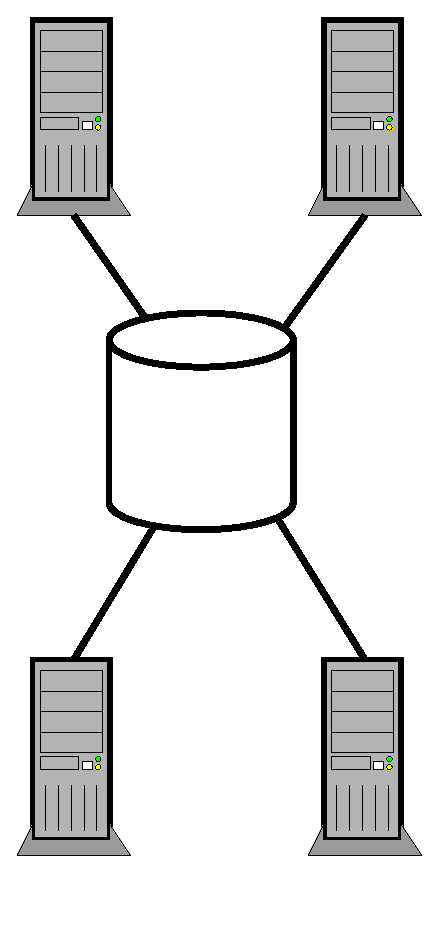
\includegraphics[width=2cm]{shared}
  \end{columns}

  $+$ Fast \\
  $-$ Limited scaling \\
  $-$ Hard to program (deadlocks, races, ...)
\end{frame}

\begin{frame}
  \frametitle{Message passing}
  
  \begin{columns}
  \column{5cm}
  Processes exchange messages.

  \column{5cm}
  \centering
  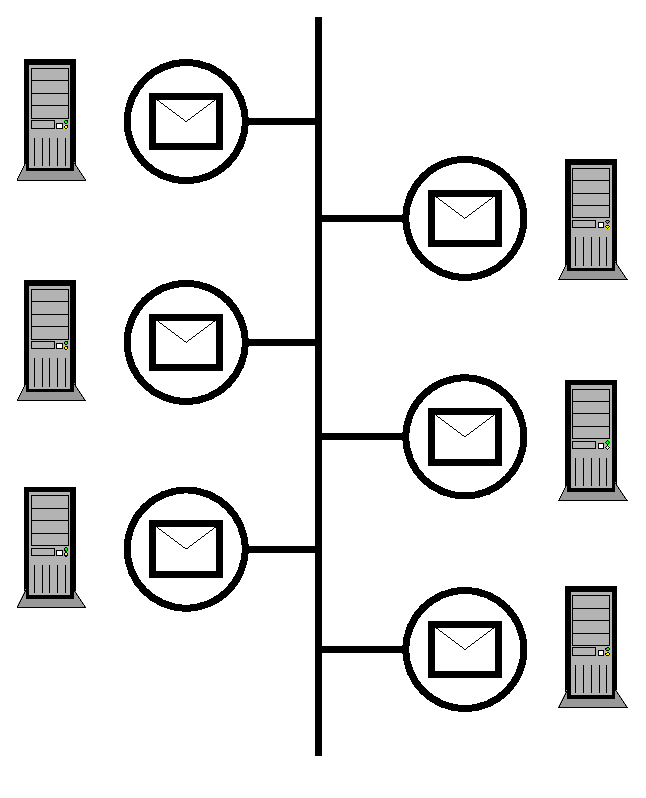
\includegraphics[width=3.5cm]{message}
  \end{columns}

  $+$ Scales well\\
  $-$ Slower \\
  $\sim$ Hard to program (easier than shared memory ?)
\end{frame}

\begin{frame}[fragile]
  \frametitle{Example (1): scala/docs/examples/actors/pingpong.scala}

  \begin{columns}
    \column{6cm}
{\tiny
\begin{verbatim}
class Ping(count: Int, pong: Actor) extends Actor {
  def act() {
    var pingsLeft = count - 1
    pong ! Ping
    loop {
      react {
        case Pong =>
          if (pingsLeft % 1000 == 0)
            println("Ping: pong")
          if (pingsLeft > 0) {
            pong ! Ping
            pingsLeft -= 1
          } else {
            println("Ping: stop")
            pong ! Stop
            exit()
          }
      }
    }
  }
}
\end{verbatim}
}

    \column{5cm}
{\tiny
\begin{verbatim}
class Pong extends Actor {
  def act() {
    var pongCount = 0
    loop {
      react {
        case Ping =>
          if (pongCount % 1000 == 0)
            println("Pong: ping "+pongCount)
          sender ! Pong
          pongCount += 1
        case Stop =>
          println("Pong: stop")
          exit()
      }
    }
  }
}
\end{verbatim}
}
  \end{columns}
\end{frame}

\begin{frame}[label=cfa]
  \frametitle{Example (2): scala/docs/examples/actors/pingpong.scala}

  \begin{columns}
    \column{5cm}
    \begin{figure}[!ht]
      \centering
      \textbf{actor$_{ping}$}
      
      \vspace{10pt}
      
      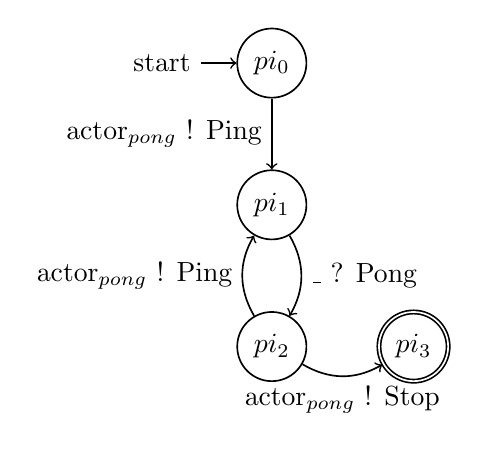
\begin{tikzpicture}[->,auto, node distance=18mm, semithick]
      \node [state,initial] (pi0) {$pi_0$};
      \node [state] (pi1) [below of=pi0] {$pi_1$};
      \node [state] (pi2) [below of=pi1] {$pi_2$};
      \node [state,accepting] (pi3) [right of=pi2] {$pi_3$};
      \path
      (pi0) edge node[left] { actor$_{pong}$ ! Ping } (pi1)
      (pi1) edge [bend left] node[right] { \_ ? Pong } (pi2)
      (pi2) edge [bend left] node[left] { actor$_{pong}$ ! Ping } (pi1)
      (pi2) edge [bend right] node[below] { actor$_{pong}$ ! Stop } (pi3)
      ;
      \end{tikzpicture}
    \end{figure}

    \column{5cm}
    \begin{figure}[!ht]
      \centering
      \textbf{actor$_{pong}$}
      
      \vspace{10pt}
      
      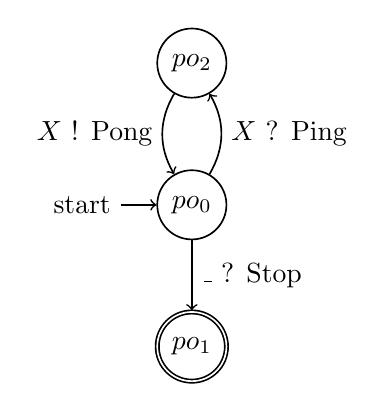
\begin{tikzpicture}[->,auto, node distance=18mm, semithick]
      \node [state,initial] (po0) {$po_0$};
      \node [state,accepting] (po1) [below of=po0] {$po_1$};
      \node [state] (po2) [above of=po0] {$po_2$};
      \path
      (po0) edge node[right] { \_ ? Stop } (po1)
      (po0) edge [bend right] node[right] { $X$ ? Ping } (po2)
      (po2) edge [bend right] node[left] { $X$ ! Pong} (po0)
      ;
      \end{tikzpicture}
    \end{figure}
  \end{columns}
\end{frame}

\begin{frame}[label=objectives]
\frametitle{Objectives and Contributions}

\begin{block}{Objectives}
\begin{itemize}
\item Identifying fragments:
\begin{itemize}
\item interesting for the programmer;
\item where verification related problems are decidable.
\end{itemize}
\item Algorithms \emph{fast enough} to check properties of those fragments.
\end{itemize}
\end{block}

\begin{block}{Contributions}
\begin{itemize}
\item An heuristic to check for Deadlock freedom of static systems.
\item A new class of dynamic systems: \alert{Star Topologies}
\item A semi-algorithm for control reachability in Star Topologies.
\end{itemize}
\end{block}

\end{frame}
%%%%%%%%%%%%%%%%%%%%%%%%%%%%%%%%%%%%%%%%%%%%
%%%%%%%%%%%%%%%%%%%%%%%%%%%%%%%%%%%%%%%%%%%%
\section{Actor Systems}

%\begin{frame}
%\frametitle{Formalism for Actor Systems}
%Having the right formalism to express\\
%a given a system of \scala{} actors.
%TODO
%\end{frame}

%%%%%%%%%%%%%%%%%%%%%%%%%%%%%%%%%%%%%%%%%%%%
\subsection{\api{}}

\begin{frame}
\frametitle{$A\pi$-calculus: Concepts}

The $\pi$-calculus \cite{DBLP:journals/iandc/MilnerPW92a,DBLP:journals/iandc/MilnerPW92b} is a process calculus able to describe concurrent computations whose configuration may change during the computation.

The \textit{asynchronous} $\pi$-calculus \cite{DBLP:conf/ecoop/HondaT91,Boudol92asynchronyand} is a restriction of the $\pi$-calculus.

\vspace{5pt}
It is build around the notions of 
\begin{description}
\item[Names]: channels as first class values. % also variables: bound
\item[Threads]: concurrent execution of parallel threads: $P\;|\;Q$.
\item[i/o prefixes]: sending/receiving messages.
\end{description}
\end{frame}

\begin{frame}[label=piSyntax]
\frametitle{$A\pi$-calculus: Syntax}
\begin{tabular}{lclr}
$P$ & ::= & $x(y).P $                           & (input prefix)\\
    & $|$ & $\overline{x} \langle y \rangle $   & (output)\\
    & $|$ & $ \sum_i a_i(b_i).P_i $             & (external choice) \\
    & $|$ & $P\;|\;P $                          & (parallel composition)\\
    & $|$ & $!P $                               & (replication) \\
    & $|$ & $(\nu x)P $                         & (name creation)\\
    & $|$ & $0 $                                & (unit process)
\end{tabular}
\end{frame}

\begin{frame}
\frametitle{$A\pi$-calculus: Example (1)}
\begin{columns}

%TODO pong Pong ping Ping
\column{5cm}
\begin{eqnarray*}
pi_0    & = & \overline{\text{pong}_{Ping}}\langle \text{ping}_{Pong} \rangle | pi_1\\
pi_1    & = & \text{ping}_{Pong}().pi_2 \\
pi_2    & = & pi_{2a} \oplus pi_{2b} \\
pi_{2a} & = & \overline{\text{pong}_{Ping}}\langle \text{ping}_{Pong} \rangle | pi_1\\
pi_{2b} & = & \overline{\text{pong}_{Stop}}\langle \rangle | pi_3 \\
pi_3    & = & 0
\end{eqnarray*}

\column{5cm}
\begin{figure}
  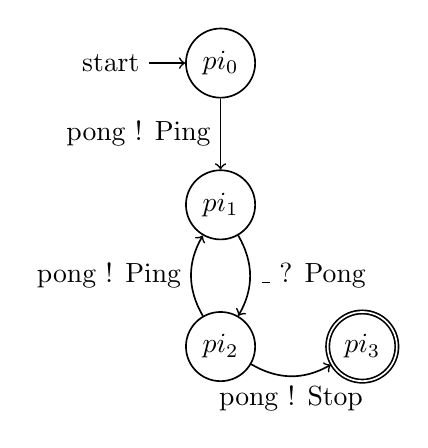
\begin{tikzpicture}[->,auto, node distance=18mm, semithick]
      \node [state,initial] (pi0) {$pi_0$};
      \node [state] (pi1) [below of=pi0] {$pi_1$};
      \node [state] (pi2) [below of=pi1] {$pi_2$};
      \node [state,accepting] (pi3) [right of=pi2] {$pi_3$};
      \path
      (pi0) edge node[left] { pong ! Ping } (pi1)
      (pi1) edge [bend left] node[right] { \_ ? Pong } (pi2)
      (pi2) edge [bend left] node[left] { pong ! Ping } (pi1)
      (pi2) edge [bend right] node[below] { pong ! Stop } (pi3)
      ;
  \end{tikzpicture}
\end{figure}
\end{columns}
\end{frame}


\begin{frame}
\frametitle{$A\pi$-calculus: Example (2)}
\begin{columns}

\column{5cm}
\begin{eqnarray*}
po_0    & = & \text{pong}_{Stop}().po_1 \\
        & + & \text{pong}_{Ping}(X).po_2\\
po_1    & = & 0 \\
po_2    & = & \overline{X}\langle \rangle | po_0
\end{eqnarray*}

\column{5cm}
\begin{figure}
  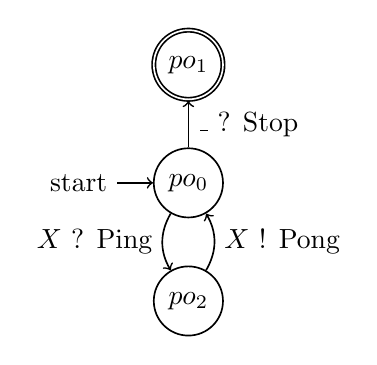
\begin{tikzpicture}[->,auto, node distance=15mm, semithick]
  \node [state,initial] (po0) {$po_0$};
  \node [state,accepting] (po1) [above of=po0] {$po_1$};
  \node [state] (po2) [below of=po0] {$po_2$};
  \path
  (po0) edge node[right] { \_ ? Stop } (po1)
  (po0) edge [bend right] node[left] { $X$ ? Ping } (po2)
  (po2) edge [bend right] node[right] { $X$ ! Pong} (po0)
  ;
  \end{tikzpicture}
\end{figure}
\end{columns}
\end{frame}

\begin{frame}
\frametitle{$A\pi$-calculus: Semantics}
Evaluating a formula in $A\pi$-calculus reduces to applying the rule:


\begin{equation*}
\alt<2>{\textcolor{red}{\overline{a}\langle b \rangle}}{\overline{a}\langle b \rangle} \;|\; \sum_{i \in I} a_i(b_i).Q_i
~~ \rightarrow ~~
\alt<3>{\textcolor{red}{Q_x[b/b_x]}}{Q_x[b/b_x]}
~~~~ \text{where $a_x = a$}
\end{equation*}

\vspace{10pt}

What happens:
\begin{itemize}
\item channel \alt<2>{\textcolor{red}{$a$ carries $b$}}{$a$ carries $b$};
\item $b$ is sent through $a$ and \alt<3>{\textcolor{red}{replace $b_x$ in the continuation $Q_x$}}{replace $b_x$ in the continuation $Q_x$}.
\end{itemize}
\end{frame}

%%%%%%%%%%%%%%%%%%%%%%%%%%%%%%%%%%%%%%%%%%%%
\subsection{General Actor Systems}

\begin{frame}
\frametitle{Overview}
The Actor Model\cite{DBLP:conf/ijcai/HewittBS73,WilliamClinger81,GulAgha86} uses \emph{actors} and their interactions to build concurrent softwares.\\

\vspace{5pt}

An actor can:
\begin{itemize}
\item send finitely many messages to other actors.
\item create a finite number of new actors.
\item receive a message from its mailbox and continue with a specified behaviour.
\end{itemize}

\vspace{10pt}

\end{frame}

\begin{frame}<1>[label=generalEq]
\frametitle{General Actor Systems}

What can an actor do ?

\vspace{5mm}

\begin{tabular}{ll}
Receive & $\displaystyle P(\vec a_I; \vec a_O) = \sum_{i \in I} a_i (\vec{b_i}).P_i(\vec a_I ;\vec a_O, \vec b_i) \hspace{3mm} \alert<2>{\forall i \in I, a_i \in \vec a_I}$ \\
Send & $P(\vec a_I; \vec a_O) = \overline{a}\langle \vec{b} \rangle | P^\prime(\vec a_I ;\vec a_O)$ \\
Branch & $P(\vec a_I; \vec a_O) = A(\vec a_I; \vec a_O) \oplus B(\vec a_I; \vec a_O)$ \\
New channel & $P(\vec a_I; \vec a_O) = (\nu \vec a).P^\prime(\vec a_I, \vec a; \vec a_O)$ \\
New actor & $P(\vec a_I; \vec a_O) = (\nu \vec n)(Q(\vec n;\emptyset) | P^\prime(\vec a_I ; \vec a_O , \vec n))$
\end{tabular}
\end{frame}

\begin{frame}
\frametitle{Unique Receiver Condition \cite{DBLP:journals/tcs/Amadio00}}
In $\pi$-calculus threads and names are independent.\\
In the actor model \alert{an actor does not share its mailbox}.

\vspace{20pt}

The unique receiver condition \alert{links channels with a thread}.
It is a syntactic restriction where names that belong to a thread are kept separately.

\end{frame}

\againframe<2>{generalEq}

\begin{frame}
\frametitle{Reachability is undecidable for General Actor Systems.}
Encoding a Turing machine into an actor system.

\begin{figure}
  \centering
  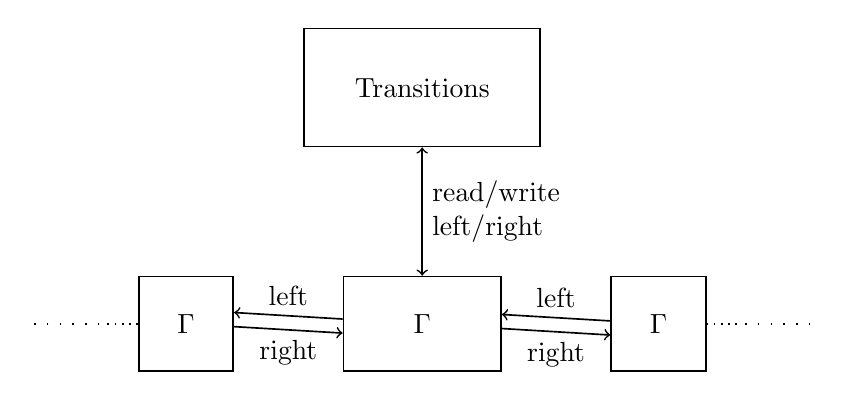
\begin{tikzpicture}[auto, node distance=3cm, semithick]

  \node[minimum width=2cm, minimum height=12mm, draw] (cells) at (0,0) {$\Gamma$};

  \node[minimum size=12mm,draw] (cLeft) [left of= cells] {$\Gamma$};
  \draw [->] (cells)[yshift=20pt]  -- node[above] { left } (cLeft);
  \draw [->] (cLeft)[yshift=-10pt] -- node[below] { right} (cells);
  
  \node[minimum size=12mm,draw] (cRight) [right of= cells] {$\Gamma$};
  \draw [->] (cRight)[yshift=10pt]  -- node[above] { left } (cells);
  \draw [->] (cells)[yshift=-20pt] -- node[below] { right} (cRight);

  \node[minimum width=3cm, minimum height=15mm, draw] (control) [above of= cells]  {Transitions};
  \draw [<->] (cells) -- node[right] {\parbox{3cm}{read/write \\ left/right}} (control);
  
  \draw [dotted] (cLeft) -- +(-1,0);
  \draw [loosely dotted] (cLeft) +(-1.1,0) -- +(-2,0);
  \draw [dotted] (cRight) -- +(1,0);
  \draw [loosely dotted] (cRight) +(1.1,0) -- +(2,0);
  \end{tikzpicture}
\end{figure}

\end{frame}

%%%%%%%%%%%%%%%%%%%%%%%%%%%%%%%%%%%%%%%%%%%%
%%%%%%%%%%%%%%%%%%%%%%%%%%%%%%%%%%%%%%%%%%%%
\section{Deadlock Freedom of {\em Static} Actor Systems}

\subsection{{\em Static} Actor Systems}
\begin{frame}
\frametitle{{\em Static} Actor Systems}

Systems of actors without creation of channels or actors are \emph{static}.
It corresponds to \api{} without creation of names.
This fragment of \api{} reduces to \pns{} \cite{DBLP:journals/njc/AmadioM02}.

\begin{rem}
Without name creation, a general \texttt{!?} + \texttt{reply} mechanism is not possible.
However, we can emulate it when there is no more than one \texttt{reply} per received message.
\end{rem}

\end{frame}


%%%%%%%%%%%%%%%%%%%%%%%%%%%%%%%%%%%%%%%%%%%%
\subsection{Petri Nets}

\begin{frame}
\frametitle{Petri Nets}

\pns{} are modeling language for discrete distributed systems.\\

A \pn{} $(S,T,F,M)$ is a directed bipartite graph where
\begin{itemize}
\item $S$ a finite set of \emph{places};
\item $T$ a finite set of \emph{transitions};
\item $F$ is the flow relation, $F \; \subseteq \; (S \times T) \bigcup (T \times S) \rightarrow \{0,1\}$ ;
\item $M$ is a marking, $M: S \rightarrow \mathbb{N}$ .
\end{itemize}
Places may contain some tokens, that are consumed and created by transitions.

\begin{figure}
  \centering
  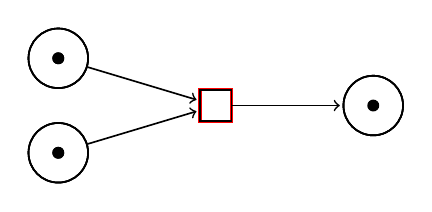
\begin{tikzpicture}[auto, node distance=2cm, semithick]

  \alt<3>{
  \node [transition] (t) at (0,0) {};
  \node [place] (a1) at (-2,0.6) {};
  \node [place] (a2) at (-2,-0.6) {};
  \node [place,tokens=1] (b) [right of= t] {};
  }{
  \alt<2>{
  \node [transition,very thick,red] (t) at (0,0) {};
  \node [place,tokens=1] (a1) at (-2,0.6) {};
  \node [place,tokens=1] (a2) at (-2,-0.6) {};
  \node [place] (b) [right of= t] {};
  }{
  \node [transition] (t) at (0,0) {};
  \node [place,tokens=1] (a1) at (-2,0.6) {};
  \node [place,tokens=1] (a2) at (-2,-0.6) {};
  \node [place] (b) [right of= t] {};
  }
  }
  \path
    (t) edge [pre] (a1)
        edge [pre] (a2)
        edge [post] (b)
  ;

  \end{tikzpicture}
\end{figure}

\end{frame}

\begin{frame}
\frametitle{Reachability: {\em Static} Actor Systems to Petri Nets (1)}
  \alt<2>{
  \begin{columns}
    \column{5cm}
    \begin{figure}[!ht]
      \centering
      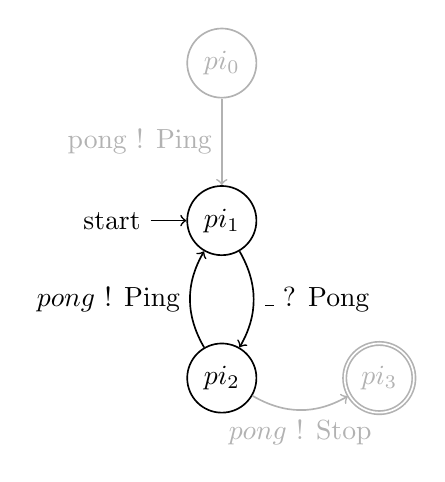
\begin{tikzpicture}[->,auto, node distance=2cm, semithick]
      \node [state,color=black!30] (pi0) {$pi_0$};
      \node [state,initial] (pi1) [below of=pi0] {$pi_1$};
      \node [state] (pi2) [below of=pi1] {$pi_2$};
      \node [state,accepting,color=black!30] (pi3) [right of=pi2] {$pi_3$};
      \path
      (pi0) edge [color=black!30] node[left] { pong ! Ping } (pi1)
      (pi1) edge [bend left] node[right] { \_ ? Pong } (pi2)
      (pi2) edge [bend left] node[left] { $pong$ ! Ping } (pi1)
      (pi2) edge [bend right,color=black!30] node[below] { $pong$ ! Stop } (pi3)
      ;
      \end{tikzpicture}
    \end{figure}

    \column{5cm}
    \begin{figure}[!ht]
      \centering
      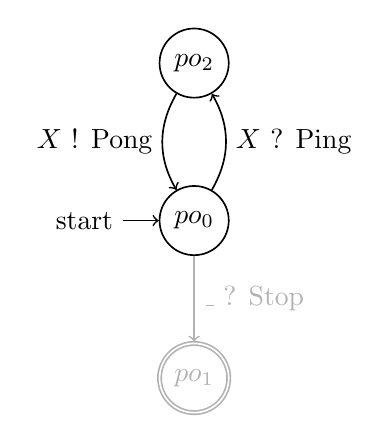
\begin{tikzpicture}[->,auto, node distance=2cm, semithick]
      \node [state,initial] (po0) {$po_0$};
      \node [state,accepting,color=black!30] (po1) [below of=po0] {$po_1$};
      \node [state] (po2) [above of=po0] {$po_2$};
      \path
      (po0) edge [color=black!30] node[right] { \_ ? Stop } (po1)
      (po0) edge [bend right] node[right] { $X$ ? Ping } (po2)
      (po2) edge [bend right] node[left] { $X$ ! Pong} (po0)
      ;
      \end{tikzpicture}
    \end{figure}
  \end{columns}
  }{
  \begin{columns}
    \column{5cm}
    \begin{figure}[!ht]
      \centering
      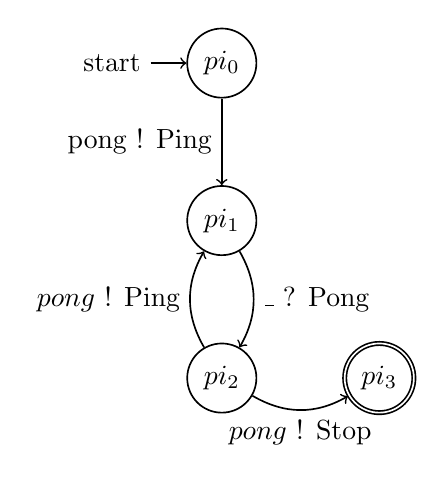
\begin{tikzpicture}[->,auto, node distance=2cm, semithick]
      \node [state,initial] (pi0) {$pi_0$};
      \node [state] (pi1) [below of=pi0] {$pi_1$};
      \node [state] (pi2) [below of=pi1] {$pi_2$};
      \node [state,accepting] (pi3) [right of=pi2] {$pi_3$};
      \path
      (pi0) edge node[left] { pong ! Ping } (pi1)
      (pi1) edge [bend left] node[right] { \_ ? Pong } (pi2)
      (pi2) edge [bend left] node[left] { $pong$ ! Ping } (pi1)
      (pi2) edge [bend right] node[below] { $pong$ ! Stop } (pi3)
      ;
      \end{tikzpicture}
    \end{figure}

    \column{5cm}
    \begin{figure}[!ht]
      \centering
      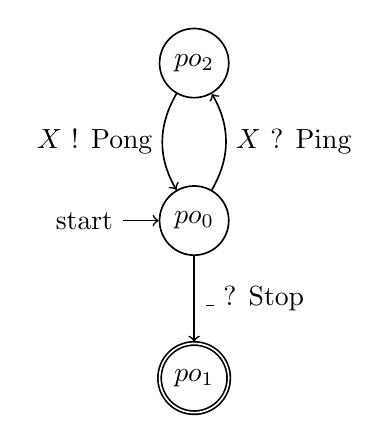
\begin{tikzpicture}[->,auto, node distance=2cm, semithick]
      \node [state,initial] (po0) {$po_0$};
      \node [state,accepting] (po1) [below of=po0] {$po_1$};
      \node [state] (po2) [above of=po0] {$po_2$};
      \path
      (po0) edge node[right] { \_ ? Stop } (po1)
      (po0) edge [bend right] node[right] { $X$ ? Ping } (po2)
      (po2) edge [bend right] node[left] { $X$ ! Pong} (po0)
      ;
      \end{tikzpicture}
    \end{figure}
  \end{columns}
  }
\end{frame}

\begin{frame}
\frametitle{Reachability: {\em Static} Actor Systems to Petri Nets (2)}
\begin{figure}[!ht]
  \centering
  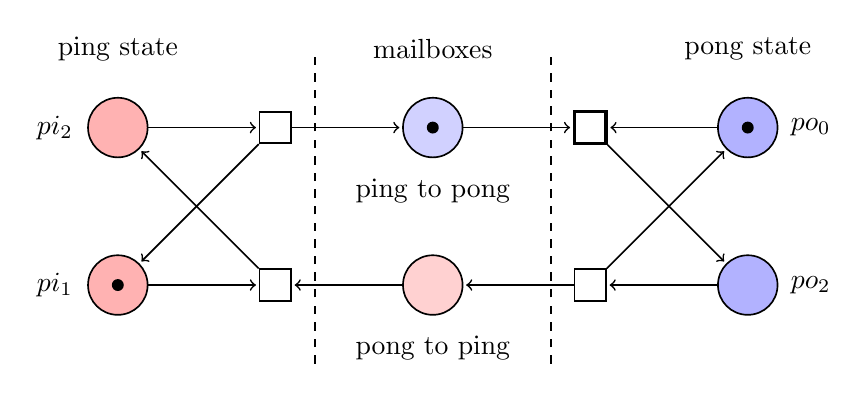
\begin{tikzpicture}[auto, node distance=2cm, semithick]

  \node (label1) at (-4,3) {ping state};
  \node (label2) at ( 0,3) {mailboxes};
  \node (label3) at ( 4,3) {pong state};
  \draw[dashed] (-1.5,-1) -- (-1.5,3);
  \draw[dashed] (1.5,-1) -- (1.5,3);

  \node [place,fill=red!18] (ping) at (0,0) {};
  \node [place,tokens=1,fill=blue!18] (pong) [above of= ping] {};

  \node [transition,very thick] (pongCatch) [right of= pong] {};
  \node [transition] (pongSend)  [below of= pongCatch] {};
  \node [place,tokens=1,fill=blue!30] (po0) [right of= pongCatch] {};
  \node [place,fill=blue!30] (po1) [below of= po0] {};
  
  \node [transition] (pingCatch) [left of = ping] {};
  \node [transition] (pingSend) [above of= pingCatch] {};
  \node [place,tokens=1,fill=red!30] (pi0) [left of= pingCatch] {};
  \node [place,fill=red!30] (pi1) [above of= pi0] {};
  \path
    (pingCatch) edge [pre] (pi0)
                edge [pre] (ping)
                edge [post] (pi1)
    (pingSend)  edge [pre] (pi1)
                edge [post] (pi0)
                edge [post] (pong)
    (pongCatch) edge [pre] (po0)
                edge [pre] (pong)
                edge [post] (po1)
    (pongSend)  edge [pre] (po1)
                edge [post] (po0)
                edge [post] (ping)
  ;

  \begin{scope}[node distance=8mm]
    \node (l1) [right of=po0] {$po_0$};
    \node (l2) [right of=po1] {$po_2$};
    \node (l3) [left of=pi0] {$pi_1$};
    \node (l4) [left of=pi1] {$pi_2$};
    \node (l5) [below of=ping] {pong to ping};
    \node (l6) [below of=pong] {ping to pong};
  \end{scope}

  \end{tikzpicture}
\end{figure}
\end{frame}
%%%%%%%%%%%%%%%%%%%%%%%%%%%%%%%%%%%%%%%%%%%%
\subsection{Structural Analysis of Petri Nets}

\begin{frame}
\frametitle{Structural Properties}

\begin{description}
\item[Siphon]: Set of places $S$ such that $ \bullet S \subseteq S \bullet $
\begin{figure}
\centering
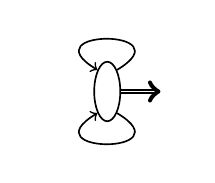
\begin{tikzpicture}[semithick]
  %\draw (0,0) arc (180:60:10pt) arc (60:-60:10pt) arc (-60:-180:10pt);
  %\draw [->] (0,0) arc (180:90:10pt);
  %\draw [->] (0,0) arc (180:-30:10pt);
  %\draw [->] (0,0) arc (180:-150:10pt);
  %\draw [->] (0,0) arc (180:60:10pt) arc (60:-60:10pt) -> +(-150:10pt);
  %\draw [->] (0,0) arc (180:60:10pt) -> +(-30:10pt);
  %\draw [->] (0,0) -> +(90:10pt);
  \node[shape=ellipse,rotate=90,draw] (a) at (0,0) {\mbox{}\hspace{3mm}\mbox{}};
  \draw [->] (a.south east) .. controls (1,0.8) and (-1,0.8) .. (a.north east) ;
  \draw [->] (a.south west) .. controls (1,-0.8) and (-1,-0.8) .. (a.north west) ;
  \draw [->,double] (a.south) -- +(0.5,0);
  \draw [->,double,transparent] (a.north)+(-0.5,0) -- (a.north);
\end{tikzpicture}
\end{figure}

\item[Trap]: Set of places $T$ such that $ T \bullet \subseteq \bullet T $.
\begin{figure}
\centering
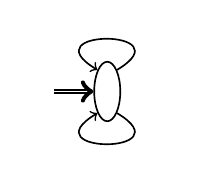
\begin{tikzpicture}[semithick]
  %\draw (0,0) arc (180:60:10pt) arc (60:-60:10pt) arc (-60:-180:10pt);
  %\draw [->] (0,0) arc (180:120:10pt);
  %\draw [->] (0,0) arc (180:0:10pt);
  %\draw [->] (0,0) arc (180:-120:10pt);
  %\draw [-<] (0,0) arc (180:60:10pt) arc (60:-60:10pt) -> +(30:10pt);
  %\draw [-<] (0,0) arc (180:60:10pt) -> +(150:10pt);
  %\draw [-<] (0,0) -> +(270:10pt);
  \node[shape=ellipse,rotate=90,draw] (a) at (0,0) {\mbox{}\hspace{3mm}\mbox{}};
  \draw [->] (a.south east) .. controls (1,0.8) and (-1,0.8) .. (a.north east) ;
  \draw [->] (a.south west) .. controls (1,-0.8) and (-1,-0.8) .. (a.north west) ;
  \draw [->,double,transparent] (a.south) -- +(0.5,0);
  \draw [->,double] (a.north)+(-0.5,0) -- (a.north);
\end{tikzpicture}
\end{figure}

\item[P-Invariant]: (nonzero integer vector $I$, integer $X$) such that
\begin{equation*}
\forall M ~\text{marking}, M_0 \rightarrow^* M: ~ \sum_{p \in P} I(p) \cdot M(p) = X
\end{equation*}
\end{description}

\end{frame}

\begin{frame}
\frametitle{Necessary Condition for Deadlock \cite{Commoner72}}
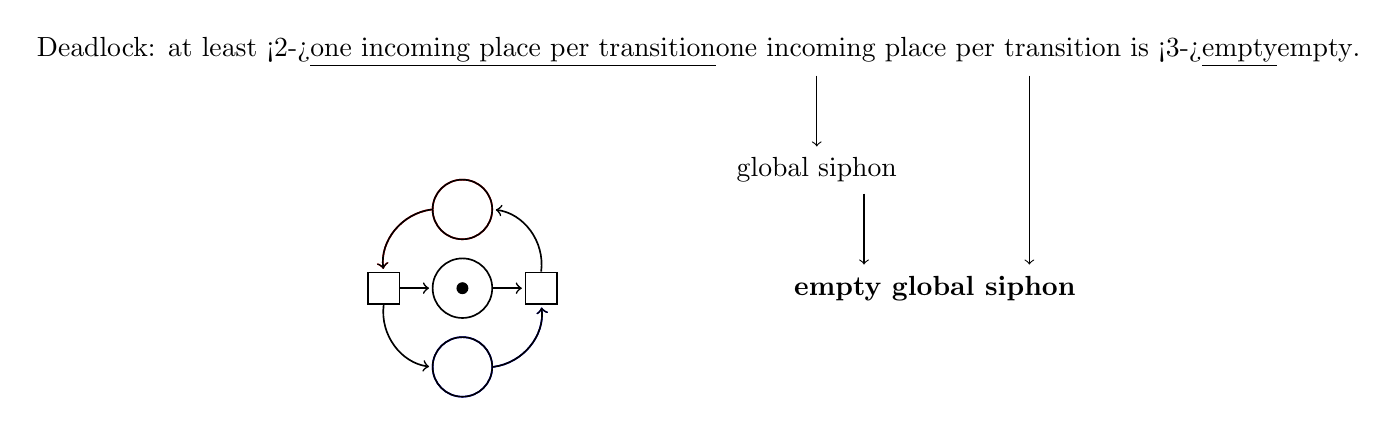
\begin{tikzpicture}
\node (text1) at (0,0) {Deadlock: at least
\alt<2->{\underline{one incoming place per transition}}{one incoming place per transition} is
\alt<3->{\underline{empty}}{empty}.};
\visible<2->{\node (text2) at (1.5,-1.5) {global siphon};}
\visible<3->{\node (text3) at (3,-3) {\textbf{empty global siphon}};}
\visible<2->{\draw [->] (1.5,-0.3) -- (1.5,-1.2);}
\visible<3->{\draw [->] (4.2,-0.3) -- (4.2,-2.7);}
\visible<3->{\draw [->] (2.1,-1.8) -- (2.1,-2.7);}

\begin{scope}[bend angle=45, semithick, xshift=-3cm, yshift=-2cm]
  \alt<3>{\node[place,red] (waiting) at (0,0) {};}{\node[place] (waiting) at (0,0) {};}
  \node[place,tokens=1]      (critical)       [below of= waiting] {};
  \alt<3>{\node[place,blue] (semaphore) [below of= critical] {};}{\node[place] (semaphore) [below of= critical] {};}
  \alt<3>{\node[transition,blue] (lc) [right of= critical] {};}{\node[transition] (lc) [right of= critical] {};}
  \draw (lc) edge [pre] (critical);
  \draw (lc) edge [post,bend right] (waiting);
  \alt<3>{\draw (lc) edge [pre, bend left,blue] (semaphore);}{\draw (lc) edge [pre, bend left] (semaphore);}
  \alt<3>{\node[transition,red] (ec) [left of= critical] {};}{\node[transition] (ec) [left of= critical] {};}
  \draw (ec) edge [post] (critical);
  \draw (ec) edge [post,bend right] (semaphore);
  \alt<3>{\draw (ec) edge [pre, bend left, red] (waiting);}{\draw (ec) edge [pre, bend left] (waiting);}
\end{scope}
\end{tikzpicture}
\end{frame}

\begin{frame}
\frametitle{Trap, Invariant, ILP, SAT}
\begin{algorithm}[H]
{\tiny
\caption{Check \pn{} for deadlock freedom}
\label{algSafePN}
\begin{algorithmic}
\REQUIRE $P = (S,T,F,M)$ a petri net %input
\ENSURE returns Yes if $P$ is deadlock free %output
\STATE $\phi \leftarrow \displaystyle \bigwedge_{s \in S} \left( s \Rightarrow \bigwedge_{t \in \bullet s} \left(\bigvee_{p \in \bullet t} p \right) \right) \land \text{\emph{finish}}$
\WHILE{ $R$ = solve($\phi$) }
\IF{ is maximal trap in $R$ marked ?}% (algorithm \ref{algMaxTrap})}
\STATE $t \leftarrow $ smallest marked trap in $R$
\STATE $\phi \leftarrow \phi \land \neg t$
\ELSIF{ $\exists (I,X)$ controlling $R$}% (algorithm \ref{algInvCtrl})}
\STATE $t \leftarrow \bigwedge_{s \in R \atop {\land I(s) \neq 0}} s$
\STATE $\phi \leftarrow \phi \land \neg t$
\ELSIF{ ILP approximation has a solution}% (algorithm \ref{algILPApprox})}
\STATE $\phi \leftarrow \phi \land \neg R$
\ELSE
\RETURN NO
\ENDIF
\ENDWHILE
\RETURN Yes
\end{algorithmic}
}
\end{algorithm}

\begin{tikzpicture}[remember picture,overlay,node distance=3cm,semithick]
  \alt<2>{
  \node [scale=0.7] (sat) at (current page.center) [above=12mm, right=17mm] {Enumerating siphons with SAT solver};
  \node (formula) at (current page.center) [above=8mm, left=7mm] {};
  \draw [->] (sat) edge (formula);
  }{
  \node [scale=0.7,transparent] (sat) at (current page.center) [above=12mm, right=17mm] {Enumerating siphons with SAT solver};
  \node (formula) at (current page.center) [above=8mm, left=7mm] {};
  }
  \alt<3>{
  \node [scale=0.7] (test) at (current page.center) [below=10mm, right=1.7cm] {Checking siphon for emptiness};
  \node (chk1) at (current page.center) [above=0mm, left=10mm] {};
  \node (chk2) at (current page.center) [below=7mm, left=14mm] {};
  \node (chk3) at (current page.center) [below=17mm, left=4mm] {};
  \draw (test.west) edge [->] (chk1);
  \draw (test.west) edge [->] (chk2);
  \draw (test.west) edge [->] (chk3);
  }{
  \node [scale=0.7,transparent] (test) at (current page.center) [below=10mm, right=1.7cm] {Checking siphon for emptiness};
  \node (chk1) at (current page.center) [above=0mm, left=10mm] {};
  \node (chk2) at (current page.center) [below=7mm, left=14mm] {};
  \node (chk3) at (current page.center) [below=17mm, left=4mm] {};
  }
  \alt<4>{
  \node [scale=0.7] (refining) at (current page.center) [below=25mm, right=1.7cm] {Refining enumeration};
  \node (ref1) at (current page.center) [below=4mm, left=12mm] {};
  \node (ref2) at (current page.center) [below=13mm, left=25mm] {};
  \node (ref3) at (current page.center) [below=20mm, left=25mm] {};
  \draw (refining.west) edge [->] (ref1);
  \draw (refining.west) edge [->] (ref2);
  \draw (refining.west) edge [->] (ref3);
  }{
  \node [scale=0.7,transparent] (refining) at (current page.center) [below=25mm, right=1.7cm] {Refining enumeration};
  \node (ref1) at (current page.center) [below=4mm, left=12mm] {};
  \node (ref2) at (current page.center) [below=13mm, left=25mm] {};
  \node (ref3) at (current page.center) [below=20mm, left=25mm] {};
  }
\end{tikzpicture}
\end{frame}

\begin{frame}
\frametitle{Example}
\begin{columns}

\column{4cm}
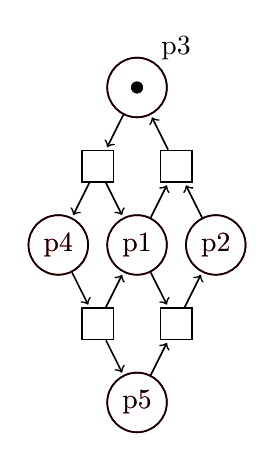
\begin{tikzpicture}[auto, node distance=1cm, semithick]

\alt<2>{\node [place,red] (p1)  at (0,0) {p1};}{\node [place] (p1)  at (0,0) {p1};}
\alt<3>{\node [place,red] (p2) at (1,0) {p2};}{\node [place] (p2) at (1,0) {p2};}
\alt<2,3>{\node [place,red,tokens=1] (p3) at (0,2) {};}{\node [place,tokens=1] (p3) at (0,2) {};}
\alt<2,3>{\node [place,red] (p4) at (-1,0) {p4};}{\node [place] (p4) at (-1,0) {p4};}
\alt<3>{\node [place,red] (p5) at (0,-2) {p5};}{\node [place] (p5) at (0,-2) {p5};}
\node [transition] (t1) at (0.5,1) {};
\node [transition] (t2) at (-0.5,1) {};
\node [transition] (t3) at (-0.5,-1) {};
\node [transition] (t4) at (0.5,-1) {};
\path
  (t1) edge [pre] (p1)
       edge [pre] (p2)
       edge [post] (p3)
  (t2) edge [pre] (p3)
       edge [post] (p4)
       edge [post] (p1)
  (t3) edge [pre] (p4)
       edge [post] (p1)
       edge [post] (p5)
  (t4) edge [pre] (p1)
       edge [pre] (p5)
       edge [post] (p2)
;
\begin{scope}[node distance=7mm]
  %\node (l1) [above right of=p1] {p1};
  %\node (l2) [above right of=p2] {p2};
  \node (l3) [above right of=p3] {p3};
  %\node (l4) [above right of=p4] {p4};
  %\node (l5) [above right of=p5] {p5};
\end{scope}
\end{tikzpicture}

\column{5cm}
\alt<4>{
\textbf{No more siphon.}\\
\pn{} is deadlock free.
}{
\alt<3>{
\textbf{Siphon p2,p3,p4,p5}\\
\begin{itemize}
\item has marked trap p2,p3,p4,p5.
\end{itemize}
}{
\alt<2>{
\textbf{Siphon p1,p3,p4}\\
\begin{itemize}
\item has no marked trap.
\item has no place invariant. 
\item has no ILP solution.
\end{itemize}
}{}}}

\end{columns}
\end{frame}

\begin{frame}
\frametitle{Results}
{\scriptsize
\begin{tabular}{l|cc|c|c|c}
Name & \#places & \#transitions & Deadlock & \textsc{Tina}\footnote{\cite{DBLP:conf/qest/BerthomieuV06}} & heuristic \\
\hline
\hline
Philo 2             & 129     & 232          & Yes      & 0.4\,s   & 0.4\,s \\
Philo 3             & 265     & 650          & Yes      & 62.4\,s  & 0.4\,s \\
Philo 4             & 449     & 1398         & Yes      & ---      & 0.6\,s \\
Philo 8             & 1665    & 9610         & Yes      & ---      & 28\,s \\
\hline
Pi approx 3         & 130     & 260          & No       & 0.2\,s   & 5.8\,s \\
Pi approx 4         & 204     & 490          & No       & 1\,s     & 137\,s \\
Pi approx 5         & 294     & 822          & No       & 11\,s    & --- \\
Pi approx 6         & 400     & 1274         & No       & 121\,s   & --- \\
Pi approx 8         & 660     & 2610         & No       & ---      & --- \\
\hline
Cell safe           & 34      & 38           & No       & ---      & 0.1\,s \\
Cell safe compact   & 4       & 26           & No       & 6.1\,s   & 0.1\,s \\
Cell unsafe         & 34      & 29           & Yes      & 0.1\,s   & 0.1\,s \\
Cell unsafe compact & 4       & 17           & Yes      & 0.1\,s   & 0.1\,s    
\end{tabular}
}

\vspace{20pt}

In our experiments we did not encounter false positives.
\end{frame}

%%%%%%%%%%%%%%%%%%%%%%%%%%%%%%%%%%%%%%%%%%%%
%%%%%%%%%%%%%%%%%%%%%%%%%%%%%%%%%%%%%%%%%%%%
\section{Extensions to {\em Dynamic} Actor Systems}

\begin{frame}
\frametitle{{\em Static} Actor Systems: Too Restrictive}

Unfortunately, most real life programs are not static.

They also \alert{create actors}.

\vspace{10pt}
We explore two cases:
\begin{itemize}
\item Parametric systems
\item Systems with creation of actors
\end{itemize}


\end{frame}

%%%%%%%%%%%%%%%%%%%%%%%%%%%%%%%%%%%%%%%%%%%%
\subsection{Parametric Systems}

\begin{frame}
\frametitle{Parametric Systems}

A parametric system is a function $\mathcal{F}$ that for any $n \in \mathbb{N}$ maps to a static system $\mathcal{F}(n)$.
The type of problem we are interested in is:

\vspace{10pt}

Given $\mathcal{F}: \mathbb{N} \rightarrow \text{Static System}$, $P$ a safety property, prove:
\begin{equation*}
\forall n \in \mathbb{N}, ~~ \mathcal{F}(n) ~\text{verifies} ~ P
\end{equation*}

\vspace{20pt}

Unfortunately, deciding such problem is in general not possible \cite{DBLP:journals/ipl/AptK86}.
\end{frame}

\begin{frame}
\frametitle{$\lim_{n \rightarrow \infty} \mathcal{F}(n)$ is Turing Complete.}
It is possible to encode a n-bounded Turing machine within $\mathcal{F}(n)$.

\begin{figure}
  \centering
  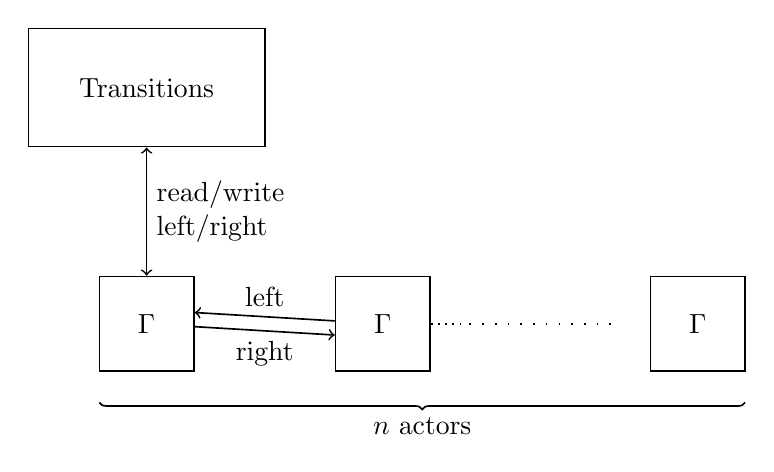
\begin{tikzpicture}[auto, node distance=3cm, semithick]

  \node[minimum size=12mm, draw] (cells) at (0,0) {$\Gamma$};
  
  \node[minimum size=12mm,draw] (cRight) [right of= cells] {$\Gamma$};
  \draw [->] (cRight)[yshift=20pt]  -- node[above] { left } (cells);
  \draw [->] (cells)[yshift=-20pt] -- node[below] { right} (cRight);
  
  \node[minimum size=12mm,draw] (cRR) at (7,0) {$\Gamma$};

  \node[minimum width=3cm, minimum height=15mm, draw] (control) [above of= cells]  {Transitions};
  \draw [<->] (cells) -- node[right] {\parbox{3cm}{read/write \\ left/right}} (control);
  
  \draw [dotted] (cRight) -- +(1,0);
  \draw [loosely dotted] (cRight) +(1.1,0) -- +(3,0);
  
  \draw [decorate,decoration={brace,mirror}] (-6mm,-10mm) -- (76mm,-10mm);
  \node[] (n) at (35mm,-13mm) {$n$ actors};
  \end{tikzpicture}
\end{figure}
\end{frame}
%%%%%%%%%%%%%%%%%%%%%%%%%%%%%%%%%%%%%%%%%%%%
\subsection{Star Topologies}

\begin{frame}
\frametitle{Star Topologies: Motivation}
What can be modeled with star topologies ?
\begin{center}
\visible<2>{\textbf{client-sever communication}}

\vspace{15pt}

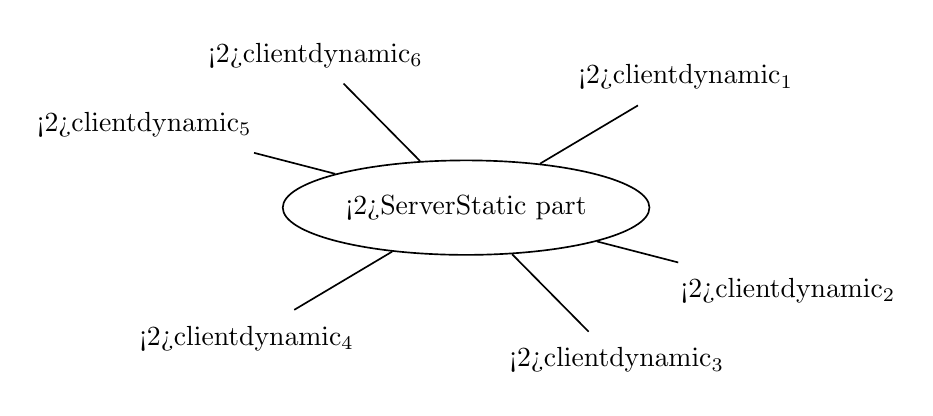
\begin{tikzpicture}[auto, semithick,
                    pin distance=10mm,
                    every pin edge/.style={black},
                    every pin/.style={minimum height=7mm, minimum width=20mm}]
\node [ellipse,draw,minimum height=12mm, minimum width=35mm,
    pin=45:{\alt<2>{client}{dynamic$_1$}},
    pin=105:{\alt<2>{client}{dynamic$_6$}},
    pin=165:{\alt<2>{client}{dynamic$_5$}},
    pin=225:{\alt<2>{client}{dynamic$_4$}},
    pin=285:{\alt<2>{client}{dynamic$_3$}},
    pin=345:{\alt<2>{client}{dynamic$_2$}}
  ]
  {\centering \alt<2>{Server}{Static part}};
\end{tikzpicture}
\end{center}
\end{frame}

\begin{frame}
\frametitle{Dynamic Creation of Actors}
\begin{block}{What we want}
Adding equations of the kind:
\begin{equation*}
P(\vec a_I; \vec a_O) = (\nu \vec n)(Q(\vec n;\emptyset) | P^\prime(\vec a_I ; \vec a_O , \vec n))
\end{equation*}
\end{block}

\vspace{20pt}
\textbf{Consequence:} 
Without any restriction, we can still apply the Turing machine construction for general actors systems.
\end{frame}

\begin{frame}
\frametitle{Restrictions}
\begin{block}{Restrictions}
\begin{itemize}
\item Limiting name mobility (1 hop)
\item Only a finite subset of all actors are allowed to create actors.
\end{itemize}
\end{block}

\vspace{10pt}

\textbf{What it does}:
Created actors are \alert{isolated} from each other.\\
(i.e. no recursive infinite structure)

\end{frame}

\begin{frame}
\frametitle{Star Topologies: Definition}
\begin{eqnarray}
P(\vec a_I; \vec a_O) & = & \sum_{i \in I} a_i (\vec{b_i}).P_i(\vec a_I ;\vec a_O, \vec b_i) \hspace{7mm} \forall i \in I, a_i \in \vec a_I \\
P(\vec a_I; \vec a_O) & = & \overline{a}\langle \vec{b} \rangle | P^\prime(\vec a_I ;\vec a_O) \hspace{20mm} \alert{\forall b \in \vec b, b \notin \vec a_O} \\
P(\vec a_I; \vec a_O) & = & A(\vec a_I; \vec a_O) \oplus B(\vec a_I; \vec a_O) \\
%P(\vec a_I; \vec a_O) & = & (\nu \vec a).P^\prime(\vec a_I, \vec a; \vec a_O) \\
\label{create} P(\vec a_I; \vec a_O) & = & (\nu \vec n)(Q(\vec n;\emptyset) | P^\prime(\vec a_I ; \vec a_O , \vec n)) 
\end{eqnarray}

\vspace{10pt}

\begin{description}
\item[Static actors] can have all types of equations, but they cannot be created.
\item[Dynamic actors] are created. However, they cannot have equations of type (\ref{create}).
\end{description}
\end{frame}

\begin{frame}
\frametitle{Star Topologies: Analysis}

%TODO why cfr and not r ?
% reset pns{}

\begin{define}[Control Flow Reachability]
Given a system of equation in $A\pi$-calculus containing an equation identifier $A$ and an initial configuration $P$,
the control flow reachability problem asks whether it is possible to reach a configuration $P^\prime$ \emph{containing} $A$:

$P \rightarrow^* P^\prime$ where $P^\prime$ is a process of the shape $\ldots | A(\ldots) | \ldots$.
\end{define}

\end{frame}

\begin{frame}
\frametitle{Star Topologies: Issues}
2 dimensions of unboundedness:
\begin{itemize}
\item unbounded number of actors;
\item unbounded number of messages in each actor's mailbox.
\end{itemize}

\vspace{20pt}

Static actor systems have only the message dimension.

\vspace{20pt}

If we can remove one dimension, we can use algorithms similar to the static case.
\end{frame}

\begin{frame}<1>[label=algo]
\frametitle{Star Topologies: Semi-algorithm}
\begin{algorithm}[H]
{\small
\caption{Control flow reachability}
\label{algCtrFlowReach}
\begin{algorithmic}
\REQUIRE $C$ a system of actors, $q$ a control flow location to cover %input
\ENSURE returns the answer to is $q$ covered in some execution of $C$ %output
\STATE $n \leftarrow 0$
\REPEAT
\STATE $n \leftarrow n+1$
\STATE $D \leftarrow \text{\dabs{}}(C,n)$
\STATE $I \leftarrow \text{\iabs{}}(C,n)$
\STATE $tree_D \leftarrow \text{coverabilityTree}(D)$
\STATE $tree_I \leftarrow \text{coverabilityTree}(I)$
\UNTIL{\alert<2>{$tree_D \approx tree_I$}}
\RETURN $q \in tree_D$
\end{algorithmic}
}
\end{algorithm}
\end{frame}

\begin{frame}
\frametitle{Star Topologies: Dual Abstraction}
Remove the messages related source of unboundedness with \alert{counter abstractions}.

\vspace{10pt}

\begin{description}
\item[\emph{drop}-counter]: 0 to bound then drop
\item[$\infty$-counter]: 0 to bound then $\infty$
\end{description}

\vspace{15pt}

\begin{description}
\item[\dabs{}] counts the messages of dynamic actors with \emph{drop}-counters.
\item[\iabs{}] counts the messages of dynamic actors with $\infty$-counters.
\end{description}
\end{frame}

\begin{frame}
\frametitle{Star Topologies: Equivalence Classes of Dynamic Actors}
Transforming a dynamic actor $d$ with an unbounded number of messages into a \alert{finite object}.

\begin{enumerate}

\item From dynamic actors to equivalence classes:
\begin{itemize}
\item Fetch all messages containing a channel owned by $d$.
\item Substitute owned channels by \texttt{Self}.
It corresponds to alpha-conversion in the $\pi$-calculus congruence relation.
\end{itemize}

\item Apply the counter abstraction on each message kind to abstract infinitely many configuration into a finite number of possibilities.

\end{enumerate}

\end{frame}

\begin{frame}
\frametitle{Star Topologies: Example of Equivalence Classes}
%TODO example of abstraction: improve ??
\begin{columns}

\column{40mm}
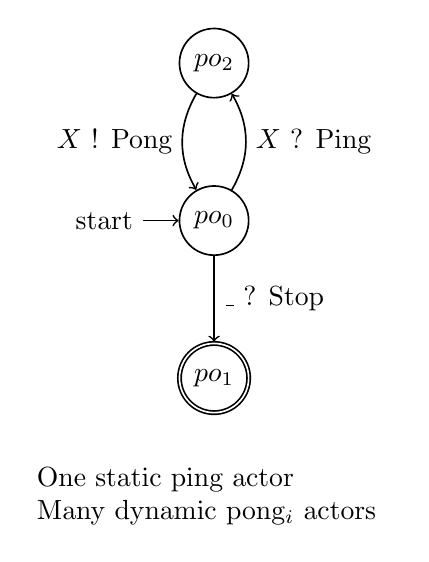
\begin{tikzpicture}[->,auto, node distance=2cm, semithick]
  \node [state,initial] (po0) {$po_0$};
  \node [state,accepting] (po1) [below of=po0] {$po_1$};
  \node [state] (po2) [above of=po0] {$po_2$};
  \path
    (po0) edge  node[right] { \_ ? Stop } (po1)
    (po0) edge [bend right] node[right] { $X$ ? Ping } (po2)
    (po2) edge [bend right] node[left] { $X$ ! Pong} (po0)
  ;
  \node[node distance=15mm] (label) [below of=po1] {\parbox{45mm}{One static ping actor\\ Many dynamic pong$_i$ actors}};
\end{tikzpicture}

\column{5cm}
\visible<4->{\alt<5>{\iabs{}}{\dabs{}}}

\begin{itemize}
\item At location $po_2$
\item Parameter $X = \text{ping}$
\item Message kinds:

\begin{tabular}{lllc}
From ~ & Type & To ~~~ & \# \\
\hline
ping & Ping & \alt<2->{\alert<2>{Self}}{pong$_n$} & 1 \\
\alt<2->{\alert<2>{Self}}{pong$_n$} & Pong & ping & \alt<5>{\alert{$\infty$}}{\alt<4>{\alert{3}}{5}}
\end{tabular}
\end{itemize}

\vspace{20pt}

\visible<3->{Bound of abstraction is 3.}

\end{columns}
\end{frame}

\begin{frame}
\frametitle{Well Structured Transition System (WSTS)}
WSTS are a generalisation of \pns{} that keep the \alert{monotonicity} properties of \pns{} \cite{DBLP:conf/lics/AbdullaCJT96,DBLP:journals/tcs/FinkelS01}.

\vspace{10pt}

The transition relation $\rightarrow$, \emph{wqo} $\leq$:
\begin{equation*}
A \leq B \land A \rightarrow A^\prime \Rightarrow \exists B^\prime. B \rightarrow B^\prime \land A^\prime \leq B^\prime
\end{equation*}

\vspace{10pt}

The property $p$ also needs to satisfy some monotonicity condition:\\
\begin{equation*}
A \text{ satisfies } p \land A \leq B \Rightarrow B \text{ satisfies } p
\end{equation*}

\end{frame}

\begin{frame}
\frametitle{Star Topologies: Coverability Tree}
Coverability Trees are used to analyse \pns{} \cite{DBLP:journals/jcss/KarpM69,DBLP:conf/apn/Finkel91}.
The idea was generalized to WSTS \cite{DBLP:conf/icalp/Finkel87}.

\begin{figure}
  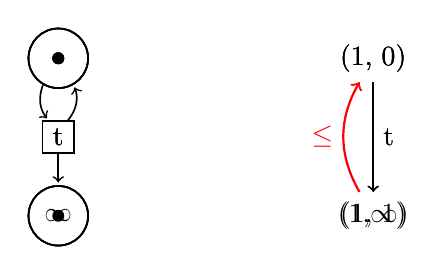
\begin{tikzpicture}[auto, node distance=1cm, semithick]

  \alt<4>{
  \node [transition] (t) at (0,0) {t};
  \node [place,tokens=1] (a) [above of= t]  {};
  \node [place] (b) [below of= t] {$\infty$};
  }{
  \alt<2-3>{
  \node [transition] (t) at (0,0) {t};
  \node [place,tokens=1] (a) [above of= t]  {};
  \node [place,tokens=1] (b) [below of= t] {};
  }{
  \node [transition] (t) at (0,0) {t};
  \node [place,tokens=1] (a) [above of= t]  {};
  \node [place] (b) [below of= t] {};
  }
  }
  \path
    (t) edge [pre, bend left] (a)
        edge [post] (b)
        edge [post, bend right] (a)
  ;
  
  \alt<4>{
  \node [] (init) at (4,1) {(1,~0)};
  \node [] (next) at (4,-1) {(1,$\infty$)};
  \draw [->] (init) edge node[right] {t} (next);
  }{
  \alt<2-3>{
  \node [] (init) at (4,1) {(1,~0)};
  \node [] (next) at (4,-1) {(1,~1)};
  \draw [->] (init) edge node[right] {t} (next);
  \visible<3>{\draw [->] (next) edge[thick,red,bend left] node[left] {$\leq$} (init);}
  }{
  \node [] (init) at (4,1) {(1,~0)};
  }
  }

  \end{tikzpicture}
\end{figure}

\end{frame}

\begin{frame}
\frametitle{Star Topologies: $\leq$}
We need a $\leq$ relation that is a well-quasi-ordering,\\
such that the control flow reachability is monotonic w.r.t. $\leq$\\
and the transition relation is also monotonic w.r.t. $\leq$.

\vspace{10pt}

$\leq$ is oriented around two axes:
\begin{itemize}
\item A configuration with more dynamic actor can do more.
\item A configuration with more messages can do more.
\end{itemize}

%TODO more details ????

\end{frame}

\begin{frame}
\frametitle{Star Topologies under-approximation: \dabs{}}

\textbf{Idea:}
With the \emph{drop}-counters some messages are removed, the rest is identical.
Furthermore, a configuration with less messages is covered by one with more messages.

\vspace{10pt}

\begin{lem}
\label{lemUnderApprox}
For all realisable paths $p_a$ in the \dabs{} $A$, there is a path $p_c$ in the corresponding concrete system $C$ such that the configurations of $p_c$ cover the configurations in $p_a$.
\end{lem}
\end{frame}

\begin{frame}
\frametitle{Star Topologies over-approximation: \iabs{}}

\textbf{Idea:}
With the $\infty$-counters messages can be added, the rest is identical.
Furthermore, a configuration were messages are added covers the original one.

\vspace{10pt}

\begin{lem}
\label{lemOverApprox}
For all realisable paths $p_c$ in a concrete system $C$, there is a path $p_a$ in the corresponding \iabs{} $A$ such that the configurations of $p_a$ cover the configurations in $p_c$.
\end{lem}
\end{frame}

\begin{frame}
\frametitle{Star Topologies: Analysis Idea}
\textbf{We have:}
\begin{center}
\dabs{} $\leq$ concrete system $\leq$ \iabs{}
\end{center}

\vspace{10pt}

\textbf{We need} a condition for:
\begin{center}
\iabs{} $\leq$ \dabs{}
\end{center}
To prove that the analysis has enough precision.
\end{frame}

\againframe<2>{algo}

\begin{frame}
\frametitle{Star Topologies: Agreement of Abstractions}
\alert{$tree_D \approx tree_I$} when:\\
\mbox{} ~~ for all path $p_i$ in the coverability tree of $I$, \\
\mbox{} ~~ there is a path $p_d$ in the coverability tree of $D$ such that
\begin{itemize}
\item both $p_i$ and $p_d$ have length $k$;
\item $\forall i \in [0,k-1]$, i$^{th}$ transition $\varphi_i$ is the same for $p_i$ and $p_d$;
\item $\forall i \in [0,k-1]$, i$^{th}$ configuration $I_i$, $D_i$ are similar ($I_i \sim D_i$).
\end{itemize}

\begin{rem}
We use $I_i \sim D_i$ and not $\leq$.
$\sim$ is defined to ignore messages of dynamic actors.
\end{rem}

\end{frame}

\begin{frame}
\frametitle{Star Topologies: Soundness}
\begin{thm}[Soundness]
\label{thmSound}
Given a system $C$, a bound $n \in \mathbb{N}$, the corresponding \dabs{} $D$ and \iabs{} $I$, and a \alert{control flow location $q$} to cover.
If the coverability trees of $D$ and $I$ agree then the answer to whether $q$ is covered can be accurately computed from the tree of $D$.
\end{thm}
\end{frame}

\begin{frame} 
  \frametitle{Conclusion}
  \begin{itemize}
  \item A General framework to express actors in $A\pi$-calculus.
  \item An efficient way of detecting deadlocks in \emph{static} systems.
  \item A new class of systems, Star Topologies, suitable to model client-server communication.
  \item A semi-algorithm to answer control flow reachability questions.
  \end{itemize}
\end{frame} 

\begin{frame} 
  \frametitle{Future Work}
  \begin{itemize}
  \item Making the agreement condition more flexible\\ (i.e. more robust w.r.t. optimisation in building the tree)
  \item Proving the completeness of the algorithm
  \item Reachability problem for star topologies
  \item Other communication topologies
  \item Is is possible to find restrictions for parametric systems ?
  \end{itemize}
\end{frame} 

\begin{frame}[allowframebreaks]{References}
  \frametitle{}
  {\tiny
  %\bibliographystyle{annotate}
  %\bibliographystyle{plainnat}
  \bibliographystyle{cell}
  %\bibliographystyle{abbrvnat}
  \bibliography{b}
  }
\end{frame}

\end{document}
